\documentclass[11pt, a4paper, titlepage, oneside]{scrbook}

\usepackage{../Tarc/Tarc}
\usepackage{../Tarc/Tarc-private}
\graphicspath{{immagini/}}

\title{Architettura degli Elaboratori}
\author{Lorenzo Ferraro}
\date{\today}
\setDegree{Informatica}

\begin{document}

\frontmatter
\SapienzaCoverItalianoTriennale
\InfoSegnalazioni

\tableofcontents

\mainmatter

\chapter{Sistemi numerici}

\section{Introduzione ai sistemi numerici}

Il sistema numerico usato normalmente è il sistema numerico \textbf{decimale} (o in base 10). In questo, ogni cifra rappresenta una potenza di \textbf{10}: $5374_{10} = 5 \cdot 10^3 + 3 \cdot 10^2 + 7 \cdot 10^1 + 4 \cdot 10^0$. Esistono, oltre a questo sistema, anche molti altri sistemi in basi diverse, tra cui il sistema \textbf{binario} e il sistema \textbf{esadecimale}.

\begin{Definizione}[Sistema binario]
\label{def-sistema-binario}
Il sistema \textbf{binario} rappresenta ogni numero tramite solo due cifre: \textbf{0} e \textbf{1}. Ogni cifra rappresenta una potenza di \textbf{2}: $1101_2 = 1 \cdot 2^3 + 1 \cdot 2^2 + 0 \cdot 2^1 + 1 \cdot 2^0 = 8 + 4 + 1 = 13_{10}$. 
\end{Definizione}

\begin{Definizione}[Sistema esadecimale]
\label{def-sistema-esadecimale}
Il sistema \textbf{esadecimale} rappresenta ogni numero tramite tutte le \textbf{10 cifre} e tramite le lettere che vanno dalla \textbf{A} alla \textbf{F} (che rappresentano i numeri da 10 a 15). Ogni cifra rappresenta una potenza di \textbf{16}: $4AF_{16} = 15 \cdot 16^0 + 10 \cdot 16^1 + 4 \cdot 16^2 =  15 + 160 + 1024 = 1199_{10}$.
\end{Definizione}

\subsection{Convertire i numeri tra i diversi sistemi numerici}

Abbiamo visto come convertire qualsiasi numero in binario/esadecimale in decimale, ma vediamo come fare il contrario.

\begin{itemize}
    \item \textbf{Decimale} $\longrightarrow$ \textbf{Binario}: vi sono due metodi:
    \begin{enumerate}[label=\arabic*°]
        \item Metodo: prendere la più grande potenza di 2 più piccola del numero da voler convertire, e sottrarla, e continuare così finché non si arriva a 0. Ad esempio, $68 = 64 - 4$, dunque $68_{10} = 1000100_2$.
        \item Metodo: dividere il numero per 2 e posizionare il resto appena ottenuto a sinistra della rappresentazione binaria. Ad esempio, $68/2 = 34 + 0 \longrightarrow 34/2 =  17 + 0 \longrightarrow 17/2 = 8 + 1 \longrightarrow 8/2 = 4 + 0 \longrightarrow 4/2 = 2 + 0 \longrightarrow 2/2 = 1 + 0 \longrightarrow 1/2 = 0 + 1$, dunque $68_{10} = 1000100_2$.
    \end{enumerate}
    \item \textbf{Decimale} $\longrightarrow$ \textbf{Esadecimale}: dividere  il numero per 16 e posizionare il resto appena ottenuto a sinistra della rappresentazione esadecimale. Ad esempio, $68/16 = 4 + 4 \longrightarrow 4/16 = 0 + 4$, dunque $68_{10} = 44_{16}$.
    \item \textbf{Esadecimale} $\longrightarrow$ \textbf{Binario}: passare da esadecimale a binario è molto semplice. Bisogna prendere ogni cifre dell'esadecimale e convertirla singolarmente in binario su 4 bit. Ad esempio, $F3A_{16} = 111100111010_2$, dato che $F = 1111$, $3 = 0011$ e $A = 1010$. Questo metodo è valido per passare da una qualsiasi base potenza di 2 al binario: basta convertire ogni cifra in un numero di bit pari all'esponente di tale potenza. Con l'esadecimale ne prendiamo 4 ($16 = 2^4$), con la base 8 invece ne usiamo solo 3 ($8 = 2^3$).
    \item \textbf{Binario} $\longrightarrow$ \textbf{Esadecimale}: anche passare da binario a esadecimale è molto semplice. Bisogna partire da destra e dividere il numero in gruppi da 4 bit. Si trasformano poi tutti i gruppi nella corrispondente cifra esadecimale e si riscrivono nello stesso ordine. Ad esempio, $100100_2 = 24_{16}$, dato che $0100_2 = 4_{16}$ e $10_2 = 2_{16}$. Questo metodo è valido per passare dal binario a una qualsiasi base potenza di 2: basta dividere il numero in gruppi di lunghezza pari all'esponente di tale potenza. Per l'esadecimale i gruppi sono lunghi 4 ($16 = 2^4$), per la base 32 sono invece lunghi 5 ($32 = 2^5$).
\end{itemize}

\begin{Proprieta}[Potenze di 2]
\label{prop-potenze-2}
Conoscendo solo alcune potenze di 2, è possibile approssimare i valori di molte più potenze. Infatti, se si conoscono tutte le potenze da $2^0$ a $2^9$, e sapendo che \mbox{$2^{10} \approx 1000, 2^{20} \approx 1000000, 2^{30} \approx 1000000000, \ldots$}, si possono approssimare tutte le potenze tra $2^0$ e $2^{39}$. Infatti, $2^{34} = 2^{30} \cdot 2^4 \approx 1000000000 \cdot 16 = 16000000000$.
\end{Proprieta}

\begin{Definizione}[Definizioni sistema binario]
\label{def-definizioni-sistema-binario}
Nel sistema binario, chiamiamo \textbf{bit} le cifre dei numeri. Un \textbf{nibble}, poi, sono 4 bit mentre un \textbf{byte} sono 8 bit. Esistono poi il \textbf{most significant bit} e \textbf{least significant bit}, che rispettivamente il bit più a sinistra e più a destra, e il \textbf{most significant byte} e \textbf{least significant byte}, che sono rispettivamente il byte più a sinistra e più a destra.  
\end{Definizione}

Ad esempio, nel numero $1010101010$, il primo 1 è il MSB, mentre l'ultimo 0 è il LSB. Allo stesso modo, nel numero CEB48E8 (rappresentato in esadecimale, dove ogni cifra rappresenta un nibble), il byte CE è il MSB, mentre il byte E8 è il LSB.

\subsection{Numeri col segno}

In qualsiasi sistema numerico, per rappresentare un numero negativo basta mettere il simbolo $-$ prima del numero. Questo, però, per i computer non è possibile: lavorando solo con dei bit, non si può anteporre ad un numero il simbolo $-$. Infatti, il computer non ha idea di cosa sia quel simbolo, conosce solo 0 e 1. Dunque bisogna trovare un'altra soluzione per rappresentare i numeri col segno. Vi sono due modi possibili:
\begin{itemize}
    \item \textbf{Segno e Ampiezza}
    \item \textbf{Completamento a 2}
\end{itemize}

\begin{Proprieta}[Segno e Ampiezza]
\label{def-Segno e Ampiezza}
\textbf{Segno e Ampiezza} è una tecnica usata dai computer per rappresentare i numeri col segno. Si usa il \textbf{bit più significativo per rappresentare il segno}: se questo vale \textbf{0}, allora il numero è \textbf{positivo}, altrimenti è \textbf{negativo}. La formula per convertire un numero in decimale è la seguente:
\[
\bm{A = (-1)^{a_{N-1}} \sum_{i = 0}^{N-2} a_i 2^i}
\]
\end{Proprieta}
Ad esempio, il numero 6 tramite il Segno e Ampiezza diventa in binario 0110, mentre -6 diventa 1110. È dunque necessario utilizzare un bit in più del normale per rappresentare i numeri. Con N bit si possono quindi rappresentare tutti i numeri da $-(2^{N-1} - 1)$ a $2^{N-1} - 1$. 

Il problema più grande di questa tecnica è l'addizione: semplicemente, questa non funziona. Se infatti proviamo a sommare -6 (1110) e 6 (0110), troviamo che
\[
\begin{array}{rccccccc}
& & & & & & \\
& & 1 & 1 & 1 & 0 & + &\\
& & 0 & 1 & 1 & 0 & = &\\
\hline
& 1 & 0 & 1 & 0 & 0& = & 19_{10} \neq 0
\end{array}
\]
Inoltre, un'altro problema è che vi sono due rappresentazioni dello 0: infatti, 0 = 1000 = 0000. 

Per questi motivi nasce un'altra tecnica, quella del \textbf{complemento a 2}.

\begin{Proprieta}[Complemento a 2]
\label{prop-complemento a 2}
\textbf{Complemento a 2} è un'altra tecnica usata per rappresentare i numeri col sengo. Il \textbf{bit più significativo} ha lo stesso valore visto con i numeri senza segno, ma con il \textbf{segno negativo}. La formula per convertire un numero in decimale è la segunete:
\[
\bm{A = a_{N-1}(-2^{N-1}) + \sum_{i = 0}^{N-2} a_i2^i}
\]
\end{Proprieta}

Ad esempio, il numero 7 tramite complemento a 2 diventa in binario 0111, mentre -7 diventa 1001. Con N bit si possono quindi rappresentare tutti i numeri da $-2^{N-1}$ a $2^{N-1} - 1$. 

Con questa implementazione si risolvono entrambi i problemi del Segno e Ampiezza. Infatti, lo zero è rappresentato solo dalla sequenza 0000, e l'addizione non ha problemi: infatti, se proviamo a sommare -6 (1010) e 6 (0110), troviamo che
\[
\begin{array}{rccccccc}
& & & & & & \\
& & 1 & 0 & 1 & 0 & + &\\
& & 0 & 1 & 1 & 0 & = &\\
\hline
& \cancel{1} & 0 & 0 & 0 & 0& = & 0
\end{array}
\]

dove l'uno inziale non si conta dato che stiamo parlando di numeri a 4 bit.

\begin{Proprieta}[Convertire un numero nell'opposto tramite il Complemento a 2]
\label{prop-trasformare-complemento-2}
Preso un numero in binario possiamo facilmente trasformarlo nell'opposto tramite il Complemento a 2. Infatti, basta \textbf{invertire i bit} e \textbf{aggiungere 1}. Preso ad esempio $6_{10} = 0110_{2}$, troviamo che $-6_{10} = 1001_2 + 1 = 1010 = -6_{10}$.
\end{Proprieta}

Questa proprietà funziona per un motivo molto semplice: sappiamo che $6 + \bar{6} = 0110 + 1001 = 1111$, dunque aggiungendo un 1 troviamo che $6 + \bar{6} + 1 = 1111 + 1 = 10000$, e dato che il primo zero si elude, troviamo che $6 + \bar{6} + 1 = 0$, ossia $-6 = \bar{6} + 1 \longrightarrow \bm{-1001 = 0110 + 1}$.  

\section{Operazioni elementari}

\subsection{Addizioni e sottrazioni}

Le addizioni in binario e in esadecimale funzionano esattamente uguale a come funzionano in decimale. Ad esempio,

\noindent
\begin{minipage}{0.48\textwidth}
\[
\begin{array}{rcccc}
& \scriptstyle 1 & & & \\
& 0 & 1 & 1 & + \\
& 0 & 1 & 0 & = \\
\hline
& 1 & 0 & 1 &
\end{array}
\]
\end{minipage}\hfill
\begin{minipage}{0.48\textwidth}
\[
\begin{array}{rcccc}
& & \scriptstyle 1 & & \\
& A & 4 & F & + \\
& 2 & A & 1 & = \\
\hline
& C & F & 0 &
\end{array}
\]
\end{minipage}

Anche per la sottrazione il metodo rimane lo stesso. Ad esempio,

\noindent
\begin{minipage}{0.48\textwidth}
\[
\begin{array}{rcccc}
& & & \scriptstyle 1 (2) & \\
& 0 & \cancel{1} \scriptstyle 0 & 0 & - \\
& 0 & 0 & 1 & = \\
\hline
& 0 & 0 & 1 &
\end{array}
\]
\end{minipage}\hfill
\begin{minipage}{0.48\textwidth}
\[
\begin{array}{rcccc}
& & & \scriptstyle 1 (16) & \\
& 3 & \cancel{D} \scriptstyle C & 9 & - \\
& 1 & A & D & = \\
\hline
& 2 & 2 & C &
\end{array}
\]
\end{minipage}

\subsection{Il problema dell'overflow}

\begin{Osservazione}[Overflow]
\label{oss-overflow}
Un problema classico nelle addizioni tra numeri binari in un sistema digitale è l'\textbf{overflow}: i computer lavorano su un numero fisso di bit, e con un addizione è possibile sforare questo numero. 
\end{Osservazione}

Ad esempio, se lavoriamo con numeri a 4 bit, la somma $1001 + 1000 = 10001$ sfora, creando diversi problemi. Infatti, con N bit abbiamo un range di numeri rappresentabili, da $0$ a $2^N-1$ (questo se parliamo di numeri senza segno).\\
Vi sono due modi per risolvere questo problema:
\begin{itemize}
    \item \textbf{Sign-Extension}
    \item \textbf{Zero-Extension}
\end{itemize}

\begin{Proprieta}[Sign-Extension]
\label{prop-sign-extention}
La \textbf{sign-extension} è un'operazione usata dai computer per aumentare il numero di bit di un numero (in Complemento a 2) così da poter completare somme su di esso che superino il limite di bit prestabilito. La regola è semplice: \textbf{duplicare il bit più significativo a sinistra raddoppiando il numero di bit del numero} (raddoppiamo il numero di bit così da esser coperti sia sulle addizioni ma anche sulle moltiplicazioni, che vedremo tra poco).
\end{Proprieta}

Ad esempio, $3_{10} = 0011 = 00000011$, e $-5_{10} = 1011 = 1111011$. Questo con gli 0 ovviamente funziona, ma anche con gli 1: infatti, $-5 = 1011 = -8 + 2 + 1 = - 16 + 8 + 2 + 1 = -32 + 16 + 8 + 2 +1 = -64 + 32 + 16 + 8 +1 = 11111011$. 

\begin{Proprieta}[Zero-Extension]
\label{zero-extension}
La \textbf{zero-extension} è un'operazione usata dai coputer per aumentare il numero di bit di un numero così da poter completare somme su di esso che superino il limtie di bit prestabilito. La regola è semplice: \textbf{raddoppiare la lunghezza del numero aggiungendo tutti 0 a sinistra}.
\end{Proprieta}
Ad esempio, $3_{10} = 0011 = 00000011$ (come nella Sign-Extension). La Zero Extension però \textbf{non funziona con i numeri col segno}. Infatti, $-5_{10} = 1011 \neq 00001011 = 11_{10}$. 

\subsection{Moltiplicazioni}

Anche le moltiplicazioni in binario e in esadecimale funzionano come in decimale. Ad esempio,

\noindent
\begin{minipage}{0.48\textwidth}
\[
\begin{array}{rccccc}
& & 0 & 1 & 1 & \times \\
& & 0 & 0 & 1 & = \\
\hline
& & 0 & 1 & 1 & + \\
& 0 & 0 & 0 & & + \\
0 & 0 & 0 & & & + \\
\hline
0 & 0 & 0 & 1 & 1
\end{array}
\]
\end{minipage}\hfill
\begin{minipage}{0.48\textwidth}
\[
\begin{array}{rccccc}
& & 3 & B & 7 & - \\
& & 2 & C & 4 & = \\
\hline
& & E & D & C & + \\
& 2 & C & 9 & & + \\
7 & 6 & E & & & + \\
\hline
A & 4 & 6 & 1 & C
\end{array}
\]
\end{minipage}

\subsection{Shift di bit}

\begin{Definizione}[Shift]
\label{def-shift}
Uno \textbf{shift} è un'operazione sui bit che \textbf{sposta tutte le posizioni dei bit} di una sequenza binaria o a destra o a sinsitra di un determinato numero di posizioni.
\end{Definizione} 

Esistono due tipi di shift:
\begin{itemize}
    \item \textbf{shift aritmetico}, dove si ripete il bit più significativo sequendo la logica della sign-extension;
    \item \textbf{shift logico}, dove si inseriscono degli 0 a sinistra della sequenza sequendo la logica della zero-extension.
\end{itemize}

Ad esempio, $-7_{10} = 1001 \bm{>>} 2 = 0010 = 2_{10}$ è uno \textbf{shift logico} (si è infatti perso il segno, cosa che capita quando si usa la zero-extension), mentre $-8_{10} = 111000 \bm{>>>} 3 = 111111 = -1_{10}$ è uno \textbf{shift aritmetico}. Notiamo che, in entrambi i casi, il nuovo numero si può ottenere prendendo l'originale e dividendolo per $2^N$, dove $N$ è il valore dello shift. Questa è una proprietà degli shift di destra. Allo stesso modo, per gli shift di sinistra, basta moltiplicare il valore per $2^N$. Ad esempio, $-8_{10} = 111000 << 2 = 100000 = -32 = -8 \cdot 2^2$.  

\begin{Proposizione}[Calcolare numero decimale dopo uno shift]
\label{propos-caloclare-decimale-post-shift}
Preso un numero $A_{10}$, effettuando uno shift a \textbf{sinistra} di $N$ posizioni, troviamo che $\bm{A_{10} << N = A_{10} \cdot 2^n}$. Se invece si effettua uno shift a \textbf{destra}, troviamo che $\bm{A >> N = A / 2^N}$.  
\end{Proposizione}

\section{Numeri con la virgola}

Siamo riusciti a rappresentare numeri interi senza segno e con il segno, ma dobbiamo ora rappresentare i \textbf{numeri con la virgola}. Abbiamo due possibili rappresentazioni: 
\begin{itemize}
    \item \textbf{Virgola fissa}
    \item \textbf{Virgola mobile}
\end{itemize}

\subsection{Rappresentazione a virgola fissa}

\begin{Proprieta}[Rappresentazione a virgola fissa]
\label{prop-rappr-virgola-fissa}
La rappresentazione a \textbf{virgola fissa} è una tecnica usata dai computer per rappresentare i numeri con la virgola. Si divide il numero in due sezioni: una rappresenta la parte intera, mentre l'altra rappresena la \textbf{parte decimale}. Il numero di bit per la parte intera e quello per la parte decimale deve essere deciso a priori. Ad ogni cifra della parte frazionaria corrisponde una \textbf{potenza di due negativa}, partendo da $2^{-1}$.
\end{Proprieta}

\Esempio \nopagebreak

Rappresentare $\bm{6.75}$ utilizzando \textbf{4 bit interi e 4 bit frazionari} (ossia per la parte decimale). \nopagebreak

Sappiamo già che $6_{10} = 0110_2$. Per la parte decimale, abbiamo 4 cifre  che ci permettono di calcolare tutti i valori da 0 a 1 con salti di $1/16$. $0.75$ diventa quindi $1100$, dato che $1100 = 1 \cdot 2^{-1} + 1 \cdot 2^{-2} = 0.5 + 0.25 =  0.75$. Dunque troviamo che $\bm{6.75 = 01101100}$.

In generale, per convertire da decimale a binario un numero con la virgola si possono usare entrambi i metodi già visti in precedenza, con una differenza per il 2° metodo: infatti, non dovremo più dividere per 2, ma dovremo moltiplicare la parte decimale per 2, e se questo numero è minore di uno allora segniamo 0, altrimenti segniamo 1 e sottraiamo 1 al valore ottenuto. Nell'esempio di prima, $0.75 \cdot 2 = 1.5 \geq 1$, dunque segniamo 1 e sottraiamo 1 ottenendo $0.5$. Ora, dato che $0.5 \cdot 2 = 1$, segniamo 1 e sottraiamo 1, ottenendo 0, dunque tutte le cifre rimanenti sono 0, e otteniamo quindi il valore $1100$.

\subsection{Numeri con la virgola con segno}

Dobbiamo ora combinare la rappresentazione a virgola fissa con il segno e ampiezza e con il complemento a 2.

\begin{itemize}
    \item Con il \textbf{segno e ampiezza} è facilissimo: semplicemente il primo bit della parte intera sarà riservato al segno.
    \item Con il \textbf{complemento a 2} bisogna utilizzare l'algoritmo visto nella Proprietà \ref{prop-trasformare-complemento-2}. 
\end{itemize}

Ad esempio, il numero $-7.5$ diventa con il segno e ampiezza $\bm{11111000}$, mentre con il complemento a 2 bisogna prima calcolare $7.5$, che è $0111000$, poi invertire i bit e sommare 1, trovando quindi come valore $\bm{10001000}$. Questo valore ha senso dato che $1 \cdot -2^3 + 1 \cdot 2^{-1} = -8 + 0.5 = -7.5$.

\begin{Proposizione}[]
\label{propos-numeri-decimali}
Utilizzare 4 bit per la parte decimale di un numero significa togliergli 4 bit per la parte intera. È quindi come se lo stessimo \textbf{dividendo per} $\bm{2^4 = 16}$. Dunque un qualsiasi numero a 8 bit con la rappresentazione a virgola fissa è pari a quello stesso numero calcolato con 8 bit di parte intera diviso per 16.
\end{Proposizione}
Riprendendo l'esempio di $-7.5$, $10001000$ con 8 bit di parte intera diventa $-120$, e infatti $-7.5 = -120/16$.

\subsection{Rappresentazione a virgola mobile}

Per studiare la rappresentazione a virgola mobile è necessario consocere la \textbf{notazione scientifica}.

\begin{Definizione}[Notazione scientifica]
\label{def-notazione-scientifica}
La \textbf{notazione scientifica} è una tecnica usata per rappresentare i numeri nella forma $\bm{\pm M \times B^E}$, dove $M$ è la \textbf{mantissa}, $B$ è la base e $E$ è l'esponente. \\
\NB In un sistema a base n, $\bm{1 \leq M < n}$. Dunque ad esempio nel sistema decimale la mantissa è compresa tra 1 e 10.
\end{Definizione}

Ad esempio, nel nostro sistema decimale scriveremmo $2437 = 2.437 \times 10^3$. 

\begin{Proprieta}[Rappresentazione a virgola mobile]
\label{prop-rappresentazione-virgola-mobile}
La rappresentazione a \textbf{virgola mobile} è una tecnica usata dai computer per rappresentare i numeri con la virgola che sfrutta la \textbf{notazione scientifica}. Si stabilisce un numero di bit a priori per rappresentare un numero, come ad esempio \textbf{32 bit}, e si dividono questi bit per rappresentare il \textbf{segno} (che richiede un bit), l'\textbf{esponente} (che, in una rappresentazione a 32 bit, richiede 8 bit) e la \textbf{mantissa} (che si prende il resto dei bit, ossia 23 in una rappresentazione a 32 bit). La base, trovandoci in un sistema binario, è ovviamente \textbf{2}.
\end{Proprieta}

Per usare questa rappresentazione bisogna:
\begin{enumerate}[label=\arabic*°]
    \item \textbf{Convertire il numero da decimale a binario}
    \item \textbf{Scriverlo nella notazione scientifica binaria} (vedremo ora come farlo)
    \item \textbf{Scriverlo nella notazione segno-esponente-mantissa}
\end{enumerate}

Vi sono però altre due importanti considerazioni da fare:
\begin{itemize}
    \item l'1 inziale della mantissa è \textbf{sottointeso}. Questo perché è sempre presente in tutti i numeri dato che $M \geq 1$.
    \item l'esponente è \textbf{polarizzato}, ossia non si usa l'esponente base ma gli si aggiunge un certo \textbf{bias}, che nel caso dei numeri a 32 bit vale 127. Questo lo si fa per poter rappresentare anche gli esponenti negativi.
\end{itemize}

\Esempio \nopagebreak

Rappresentare il numero $\bm{-228}_{10}$ usando la \textbf{rappresentazione a virgola mobile con 32 bit}. \nopagebreak

Per prima cosa, quindi, convertiamo $228$ in binario (il segno non ci interessa, vi è un bit apposta in questa rappresentazione che se ne occupa): $228_{10} = 11100100_2$. A questo punto dobbiamo scriverlo nella notazione scientifica binaria, in un processo che prende il nome di \textbf{normalizzazione}: $11100100_2 = 1.11001_2 \times 2^7$. Aggiungiamo il bias all'esponente che diventa $127 + 7 = 134$, e riscriviamo tale numero nella sua rappresentazione a 32 bit finale:
\[
1 | 10000110 | 11001000000000000000000_2
\]

il cui valore esadecimale è $0xC3640000$ (dove $0x$ indica l'inizio del valore esadecimale).

Vi sono diverse convenzioni da stabilire per questa rappresentazione, dunque si utilizza uno standard che prende il nome di \textbf{IEEE 754}.

\begin{Definizione}[IEEE 754]
\label{def-IEEE754}
L'\textbf{IEEE 754} è lo standard utilizzato per la rappresentazione a virgola mobile.
\end{Definizione}

Racchiudiamo in questa tabella tutti i casi speciali della rappresentazione a virgola mobile, che sono stati così standardizzati sotto l'IEEE 754.

\begin{center}
\begin{tabular}{|l|c|c|l|}
\hline
Number & Sign & Exponent & Fraction \\
\hline
\textbf{0} & Indifferente & 00000000 & 00000000000000000000000 \\
\hline
$\bm{\infty}$ & 0 & 11111111 & 00000000000000000000000 \\
\hline
$\bm{-\infty}$ & 1 & 11111111 & 00000000000000000000000 \\
\hline
\textbf{NaN} & Indifferente & 11111111 & non-zero \\
\hline
\textbf{Denormalizzati} & Indifferente & 00000000 & $M \neq 0$ \\
 & & & $(-1)^s \times 2^{-126} \times 0.m$ \\
\hline
\end{tabular}
\end{center}

Dunque lo 0 si rappresenta con il codice esadecimale 0x00000000 o il codice 0x80000000 (vi sono anche qui, come nel Segno e Ampiezza, due rappresentazioni per esso). \\
Quando invece vogliamo rappresentare un operazione indefinita, come $\infty - \infty$ o $0/0$. \\
Nella tabella sono anche rappresentati un altro genere di numeri: i numeri \textbf{denormalizzati} (o subnormali). Questi numeri sono numeri la cui mantissa non inizia con 1, perché voglio rappresentare numeri ancora più piccoli di $10^{-126}$ (che sarebbe il minimo consentito dai numeri normalizzati dato che l'esponente 00000000 è riservato allo 0). Infatti, si è pensato che dividendo il valore della mantissa per $2$ si potesse diminuire ancora di più. Ad esempio, $0.1 \times 10^{-126}$ ha sempre come esponente $-126$, ma ha come mantissa $0.1$ e non $1$. In questo caso, però, si deve quindi togliere l'1 sottinteso di cui avevamo parlato precedentemente, e si perde anche precisione: infatti i bit rimanenti per la mantissa vera e propria diminuiscono sempre di più a favore di numeri più piccoli. In questo modo, però, è possibile arrivare fino a $2^{-149}$ con soli 32 bit.

\begin{Proprieta}[Livello di precisione]
\label{prop-livello-di-precisione}
In base al numero di bit, si può raggiungere un livello di precisione più o meno alto. Vi sono 3 standard conosciuti:
\begin{itemize}
    \item \textbf{Half-Precision} (16 bit)
    \item \textbf{Single-Precision} (32 bit, ciò che utilizzeremo noi)
    \item \textbf{Double-Precision} (64 bit)
\end{itemize}
\end{Proprieta}

\subsection{Arrotondare numeri a virgola mobile}

Abbiamo già affrontato il problema dell'overflow, ossia quando un numero sfora il numero di bit consenti (esiste poi anche l'\textbf{underflow}, ossia quando un numero è così piccolo da non poterlo rappresentare). Questo problema è risolvibile in parte grazie alla sign-extension o alla zero-extension, ma ci sono numeri che da un sistema binario non sono rappresentabili. Ad esempio, $1/3$ non è rappresentabile: si avrebbe bisogno di un numero di bit infinito. È per questo che in informatica spesso bisogna \textbf{arrotondare}.

\begin{Proprieta}[Arrotondare]
\label{prop-arrotondare}
Esistono quattro modi per arrotondare un numero:
\begin{enumerate}
    \item per \textbf{difetto}
    \item per \textbf{eccesso}
    \item più \textbf{vicino allo zero} (ossia se è positivo per difetto, se è negativo per eccesso)
    \item al \textbf{più vicino possibile} (default, e in caso di parità arrotonda al valore il cui bit meno significativo è pari, ossia 0)
\end{enumerate}
\end{Proprieta}

Per capire meglio questi concetti, vediamo come arrotondare $1.100101$ ($1.578125$) a solo 3 bit dopo la virgola con tutti e 4 i modi.

\begin{enumerate}
    \item $\bm{1.100}$
    \item $\bm{1.101}$
    \item $\bm{1.100}$
    \item $\bm{1.101}$ (dato che la parte scartata $101$ è maggiore della metà dell'intervallo $100$)
\end{enumerate}

\subsection{Addizione con i numeri in virgola mobile}

L'addizione tra numeri in virgola mobile segue dei passaggi molto specifici:
\begin{enumerate}[label=\arabic*°]
    \item Si estraggono l'esponente e i bit frazionari
    \item Si comparano gli esponenti, e si shifta la mantissa più piccola se necessario
    \item Si sommano le mantisse
    \item Si normalizza la mantissa e si aggiusta l'esponente se necessario
    \item Si arrotonda il risultato
    \item Si riscrive il numero nel formato a virgola mobile
\end{enumerate}

Può sembrare difficile, ma vediamo un esempio per chiarirci le idee. Sommiamo i numeri $0x3FC00000$ e $0x40500000$.

Per prima cosa dobbiamo quindi estrarre l'esponente e i bit frazionari di entrambi i numeri:
\begin{align*}
3FC00000_{16} &= 0|01111111|10000000000000000000000 \\
40500000_{16} &= 0|10000000|10100000000000000000000
\end{align*}

La mantissa del primo numero è quindi $1.1$, mentre per il secondo è $1.101$. Gli esponenti sono rispettivamente $127$ e $128$, ossia $0$ e $1$ tolto il bias, e dato che $0 - 1= - 1$, dobbiamo fare uno shift verso destra della mantissa del primo numero di 1. Dunque $1.1 >> 1 = 0.11 \ (\times 2^1)$. Possiamo ora sommare le due mantisse:

\[
\begin{array}{rccccc}
& & 0. & 1 & 1 & + \\
& 1 & 1 & 0 & 1 & = \\
\hline
1 & 0. & 0 & 1 & 1 &
\end{array}
\]

Dobbiamo ora normalizzare la mantissa: $10.011 \times 2^1 = 1.0011 \times 2^2$. Non serve arrotondare nulla, dato che i bit frazionari sono ben meno di 23, dunque possiamo riscrivere tutto nel formato a virgola mobile:
\[
0|10000001|00110000000000000000000 = 0x4098000_{16}
\]

Se invece prendiamo due numeri con segno opposto, come ad esempio $0x40C00000$ e $0xC0200000$. 

Per prima cosa estraiamo l'esponente e i bit frazionari:
\begin{align*}
40C00000_{16} &= 0|10000001|10000000000000000000000 \\
C0200000_{16} &= 1|10000000|01000000000000000000000
\end{align*}

La mantissa del primo numero è $1.1$, mentre quella del secondo è $1.01$. Gli esponenti sono rispettivamente $129$ e $128$, ossia $2$ e $1$, e dato che $2-1 = 1$, dobbiamo fare uno shift verso destra della mantissa del secondo numero di 1. Dunque $1.01 >> 1 =  0.101 \ (\times 2^2)$. Possiamo ora sottarre (dato che la seconda è negativa) le due mantisse :

\[
\begin{array}{rcccc}
1. & 0 & 0 & 0 & - \\
0. & 1 & 0 & 1 & = \\
\hline
0. & 1 & 1 & 1 &
\end{array}
\]

Dobbiamo ora normalizzare la mantissa: $0.111 \times 2^2 = 1.11 \times 2^1$. Non dobbiamo arrotondare nulla, quindi possiamo riscrivere tutto nel formato a virgola mobile:
\[
0|10000000|11000000000000000000000 = 0x40600000
\]

\subsection{Moltiplicazione con numeri in virgola mobile}

Anche la moltiplicazione tra numeri in virgola mobile è abbastanza schematica:
\begin{enumerate}[label=\arabic*°]
    \item Si estraggono gli esponenti e i bit frazionari
    \item Si sommano gli esponenti (togliendo poi un bias, dato che sennò ne avremmo due)
    \item Si fa il prodotto tra le mantisse
    \item Si calcola il segno (se i segni sono discordi allora è -, altrimenti è +)
    \item Si normalizza il tutto se necessario
    \item Si riscrive il numero nel formato a virgola mobile
\end{enumerate}

Proviamo a moltiplicare $0x4040000$ e $0x40200000$.

Per prima cosa estraiamo quindi l'esponente e i bit frazionari da entrambi i numeri:
\begin{align*}
40400000_{16} &= 0|10000000|10000000000000000000000 \\
40200000_{16} &= 0|10000000|01000000000000000000000
\end{align*}

La mantissa del primo numero è 1.1, mentre quella del secondo è 1.01. Gli esponenti sono entrambi 128, dunque l'esponente finale è $128+128-127 = 129$. Eseguiamo ora il prodotto tra le mantisse:
\[
\begin{array}{rccccc}
& & 1. & 1 & 0 & \times \\
& & 1. & 0 & 1 & = \\
\hline
& & 1 & 1 & 0 & + \\
& 0 & 0 & 0 & & \\
1 & 1 & 0 & & & = \\
\hline
1. & 1 & 1 & 1 & 0
\end{array}
\]
Non dovendo normalizzare nulla, possiamo riscrivere tutto nel formato a virgola mobile:
\[
0|10000001|11100000000000000000000 = 0x40F00000
\]

\chapter{Circuiti logici}

\section{Funzioni logiche}

\begin{Definizione}[Funzione logica]
\label{def-funzione-logica}
Una \textbf{funzione logica} (o booleana) è una funzione matematica definita su variabili binarie (ossia che possono valere solo 0 o 1, dove 0 = Falso e 1 = Vero) che restituisce a sua volta un valore di 0 o 1 in uscita.
\end{Definizione}

Esistono diverse funzioni logiche:
\begin{itemize}
    \item Funzioni logiche a un input: \codeb{NOT} \textbf{gate, buffer}
    \item Funzioni logiche a più input: \codeb{AND, OR, XOR, NAND, NOR, XNOR}
\end{itemize}

Useremo spesso le \textbf{tabelle di verità} per comprendere come funzionano queste funzioni logiche.

\subsection{Funzioni logiche a un input}

\begin{minipage}[c]{0.35\textwidth}
\centering
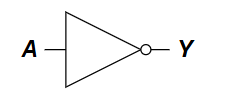
\includegraphics[width=1\textwidth, valign=t]{NOT Logico.png}
\end{minipage}\hfill
\begin{minipage}[c]{0.60\textwidth}
Il \codeb{NOT} \textbf{gate} si rappresenta tramite un trinagolo con un pallino finale (questo pallino lo vedremo con qualsiasi funzione che utilizza l'operatore \code{NOT} per negare qualcosa). In questo caso abbiamo $\bm{Y = \bar{A}}$ (indichiamo con una barretta l'inverso di una variabile, dunque se $A$ è 0 $\bar{A} = 1$ e viceversa), che si rappresenta così tramite la tabella di verità:

\[
\begin{array}{c|c}
A & Y \\
\hline
0 & 1 \\
1 & 0
\end{array}
\]

Dunque il \code{NOT} gate \textbf{inverte il valore in input}.
\end{minipage}

\begin{minipage}[c]{0.35\textwidth}
\centering
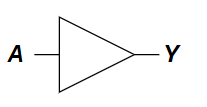
\includegraphics[width=1\textwidth, valign=t]{Buffer.png}
\end{minipage}\hfill
\begin{minipage}[c]{0.60\textwidth}
Il \textbf{buffer} si rappresenta tramite un trinagolo. In questo caso abbiamo $\bm{Y = A}$, che si rappresenta così tramite la tabella di verità:

\[
\begin{array}{c|c}
A & Y \\
\hline
1 & 0 \\
1 & 0
\end{array}
\]

Dunque il buffer \textbf{lascia invariato il valore in input}
\end{minipage}

\subsection{Funzioni logiche a più input}

\begin{minipage}[c]{0.35\textwidth}
\centering
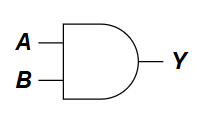
\includegraphics[width=1\textwidth, valign=t]{AND logico.png}
\end{minipage}\hfill
\begin{minipage}[c]{0.60\textwidth}
L'\codeb{AND} si rappresenta tramite un rettangolo unito a un semicerchio. In questo caso abbiamo $\bm{Y = AB}$, che si rappresenta così tramite la tabella di verità:

\[
\begin{array}{cc|c}
A & B & Y \\
\hline
0 & 0 & 0 \\
0 & 1 & 0 \\
1 & 0 & 0 \\
1 & 1 & 1
\end{array}
\]

Dunque l'\code{AND} ritorna vero se \textbf{entrambi i valori sono veri}.
\end{minipage}

\begin{minipage}[c]{0.35\textwidth}
\centering
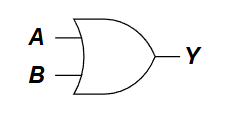
\includegraphics[width=1\textwidth, valign=t]{OR Logico.png}
\end{minipage}\hfill
\begin{minipage}[c]{0.60\textwidth}
L'\codeb{OR} si rappresenta tramite tre archi uniti a formare una specie di triangolo. In questo caso abbiamo $\bm{Y = A + B}$, che si rappresenta così tramite la tabella di verità:

\[
\begin{array}{cc|c}
A & B & Y \\
\hline
0 & 0 & 0 \\
0 & 1 & 1 \\
1 & 0 & 1 \\
1 & 1 & 1
\end{array}
\]

Dunque l'\code{OR} ritorna vero se \textbf{almeno uno dei due valori è vero}.
\end{minipage}

\begin{minipage}[c]{0.35\textwidth}
\centering
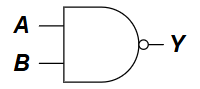
\includegraphics[width=1\textwidth, valign=t]{NAND Logico.png}
\end{minipage}\hfill
\begin{minipage}[c]{0.60\textwidth}
Il \codeb{NAND} si rappresenta con la stessa figura dell'\code{AND} ma termina con un pallino. In questo caso abbiamo $\bm{Y = \overline{AB}}$, che si rappresenta così tramite la tabella di verità:

\[
\begin{array}{cc|c}
A & B & Y \\
\hline
0 & 0 & 1 \\
0 & 1 & 1 \\
1 & 0 & 1 \\
1 & 1 & 0
\end{array}
\]

Dunque il \code{NAND} ritorna vero se \textbf{almeno uno dei due valori è falso} (il contrario dell'\code{AND}).
\end{minipage}

\begin{minipage}[c]{0.35\textwidth}
\centering
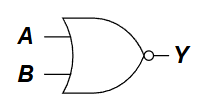
\includegraphics[width=1\textwidth, valign=t]{NOR Logico.png}
\end{minipage}\hfill
\begin{minipage}[c]{0.60\textwidth}
Il \codeb{NOR} si rappresenta con la stessa figura dell'\code{OR} ma termina con un pallino. In questo caso abbiamo $\bm{Y = \overline{A + B}}$, che si rappresenta così tramite la tabella di verità:

\[
\begin{array}{cc|c}
A & B & Y \\
\hline
0 & 0 & 1 \\
0 & 1 & 0 \\
1 & 0 & 0 \\
1 & 1 & 0
\end{array}
\]

Dunque il \code{NOR} ritorna vero se \textbf{entrambi i valori sono falso} (il contrario dell'\code{OR}).
\end{minipage}

\begin{minipage}[c]{0.35\textwidth}
\centering
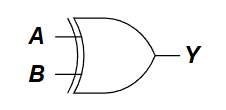
\includegraphics[width=1\textwidth, valign=t]{XOR Logico.png}
\end{minipage}\hfill
\begin{minipage}[c]{0.60\textwidth}
Lo \codeb{XOR} si rappresenta con la stessa figura dell'\code{OR} ma ha un doppio arco alla base. In questo caso abbiamo $\bm{Y = A \oplus B}$, che si rappresenta così tramite la tabella di verità:

\[
\begin{array}{cc|c}
A & B & Y \\
\hline
0 & 0 & 0 \\
0 & 1 & 1 \\
1 & 0 & 1 \\
1 & 1 & 0
\end{array}
\]

Dunque il \code{XOR} ritorna vero se \textbf{i due valori sono diversi}.
\end{minipage}

\begin{minipage}[c]{0.35\textwidth}
\centering
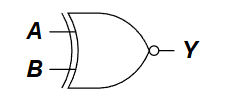
\includegraphics[width=1\textwidth, valign=t]{XNOR Logico.png}
\end{minipage}\hfill
\begin{minipage}[c]{0.60\textwidth}
Lo \codeb{XNOR} si rappresenta con la stessa figura dello \code{XOR} ma termina con un pallino. In questo caso abbiamo $\bm{Y = \overline{A \oplus B}}$, che si rappresenta così tramite la tabella di verità:

\[
\begin{array}{cc|c}
A & B & Y \\
\hline
0 & 0 & 0 \\
0 & 1 & 1 \\
1 & 0 & 1 \\
1 & 1 & 0
\end{array}
\]

Dunque il \code{XNOR} ritorna vero se \textbf{i due valori sono uguali} (il contrario dello \code{XOR}).
\end{minipage}

\begin{Proprieta}[Proprietà dispari dello \code{XOR}]
\label{prop-proprietà-dispari-XOR}
Prese tante variabili booleane $X_1, \ldots, X_n$, 
\[
X_1 \oplus \ldots \oplus X_n = \begin{cases}
    \bm{1} & \textbf{se il numero di 1 è dispari} \\
    \bm{0} & \textbf{se il numero di 1 è pari} 
\end{cases}
\]
Possiamo quindi dire che ogni 1 aggiunto allo \code{XOR} \textbf{inverte} il risultato.
\end{Proprieta}

\Dimostrazione \nopagebreak

Dimostreremo questa proprietà solo con 3 variabili, ma vale con una qualsiasi somma di $n$ variabili. \\
Prese $A,B,C$, essendo lo XOR associativo sappiamo che $A \oplus B \oplus C = (A \oplus B) + C$. Poniamo $Y = A \oplus B$. Dunque
\[
Y \oplus C =
\begin{cases}
Y & \text{se } C = 0 \\
\overline{Y} & \text{se } C = 1 
\end{cases}
\]

Dunque se $C = 0$, allora avremo che $A \oplus B \oplus C = A \oplus B$ che vale $0$ se il numero di 1 è pari e $1$ se invece è dispari. Se invece $C = 1$, allora avremo che $A \oplus B \oplus C = \overline{A \oplus B}$ che vale $0$ se il numero di 1 è dispari e $1$ se invece è pari. Dunque ogni $1$ che si aggiunge allo \code{XOR} inverte il risultato. $\blacksquare$

\section{Circuiti logici}

\begin{Definizione}[Circuito logico]
\label{def-circuito-logico}
Un \textbf{circuito logico} è un circuito elettrico digitale dotato di una serie di input e output che elaborano segnali binari.
\end{Definizione}
Il comportamento logico è descritto dalla \textbf{specifica funzionale}, che descrive cosa fa il circuito. Inoltre, è a volte presente una \textbf{specifica temporale}, che ne ritarda le operazioni per poter decidere quando far restituire l'output.

Un circuito logico è formato da due elementi fondamentali:
\begin{itemize}
    \item I \textbf{nodi} rappresentano i fili che trasportano il segnale binario, e possono essere ingressi, uscite o nodi interni.
    \item Gli \textbf{elementi del circuito} sono i blocchi logici che formano un circuito, e possono essere una singola porta logica o altri sotto-circuiti.
\end{itemize}

Esistono due tipi di circuiti logici:
\begin{itemize}
    \item \textbf{Circuiti combinatori}, che non hanno memoria e il cui output è determinato solo dai valori di input correnti
    \item \textbf{Circuiti sequenziali}, che invece hanno memoria e il cui output dunque è determinato non solo dai valori correnti ma anche quelli passati
\end{itemize}

Un esempio classico di circuiti sequenziali è la macchinetta delle bevande: se si vuole prendere la bevanda indicata con il numero 34, bisognerà schiacciare prima il 3 e poi il quattro. Ma noi non schiacciamo i tasti in contemporanea, ma in modo sequenziale. Dunque abbiamo bisogno di un circuito che si ricordi che abbiamo premuto prima il 3 e poi il 4, e non che dimentichi tutto ogni volta.

\begin{Proprieta}[Regole dei circuiti combinatori]
\label{prop-regole-circuiti-combinatori}
Ci sono diverse regole da rispettare per creare dei circuiti combinatori funzionanti:
\begin{enumerate}
    \item ogni elemento è \textbf{combinatorio}
    \item ogni nodo è o un \textbf{input} o è \textbf{collegato all'output di un solo componente interno}
    \item il circuito \textbf{non ha cicli}
\end{enumerate}
\end{Proprieta}

\begin{minipage}[c]{0.35\textwidth}
\centering
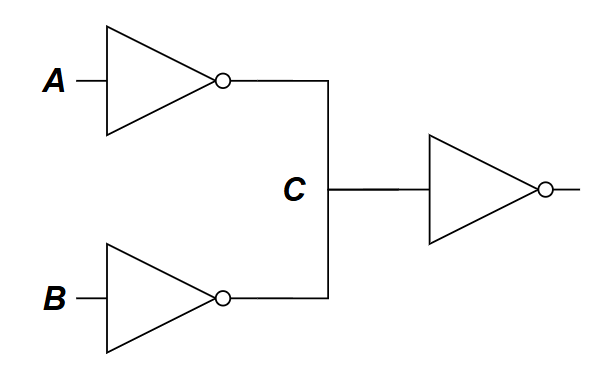
\includegraphics[width=1\textwidth, valign=t]{Circuito combinatorio errato.png}
\end{minipage}\hfill
\begin{minipage}[c]{0.60\textwidth}
Questo ad esempio non è un circuito combinatorio corretto. Infatti, il nodo \codeb{C} si trova in un valore intermedio non determinato: non sappiamo se vale 1 o 0 dato che non vi è nessuna porta logica che prenda in input i due valori $\bar{A}$ e $\bar{B}$ per creare un unico output sensato. Il nodo \code{C} è quindi \textbf{collegato all'output di due componenti interni}, violando così la regola 2).
\end{minipage}

\begin{minipage}[c]{0.35\textwidth}
\centering
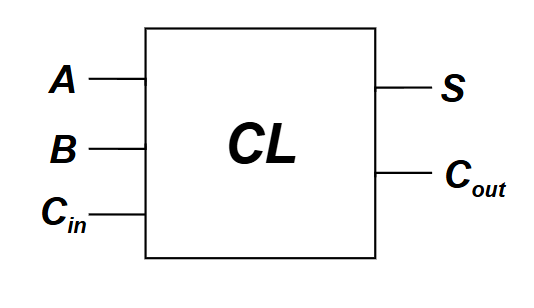
\includegraphics[width=1\textwidth, valign=t]{Circuito CL esempio.png}
\end{minipage}\hfill
\begin{minipage}[c]{0.60\textwidth}
Questo invece è uno dei circuiti combinatori dell'architettura degli elaboratori: si chiama \textbf{Full Adder} e serve per eseguire delle somme di bit. In questo caso prendiamo i due bit da sommare $A$ e $B$ e il riporto proveniente da un'eventuale somma precedente $C_{in}$. L'output è $S = A \oplus B \oplus C_{in}$, che sarebbe la somma tra bit, e $C_{out}$, l'evenutale riporto generato.\\
\NB Il blocco CL centrale indica un circuito logico. Si potrebbe pensare che in questo caso avremmo potuto mettere uno \code{XOR} a 3 input, ma questo non funziona: infatti, uno \code{XOR} rilascia solo un output, mentre noi in questo caso abbiamo un circuito che rilascia due output. Dunque creiamo questo blocco CL che rappresenta un circuito logico di cui i dettagli implementativi non ci interessano.
\end{minipage}


\section{Equazioni booleane}

\begin{Definizione}[Equazioni booleane]
\label{def-equazioni-booleane}
Un'\textbf{equazione booleana} è un'uguaglianza matematica tra due espressioni composte da variabii booleane e operatori logici.
\end{Definizione}

\begin{Definizione}[Definizioni dell'algebra di Boole]
\label{def-algebra-boole}
L'\textbf{algebra di Boole} è quella branca dell'algebra che si occupa di studiare le equazioni booleane. Vi sono diversi termini necessari da conoscere per poterla studiare:
\begin{itemize}
    \item \textbf{Complemento}: una variabile con una barra ($\bar{A}$)
    \item \textbf{Literal}: una variabile o il suo complemento ($A$ o $\bar{B}$)
    \item \textbf{Implicante}: un prodotto tra literal ($AC$ o $A \bar{B}$)
    \item \textbf{Mintermine}: un prodotto che include tutte le variabili in input ($AB\bar{C}$, se come input abbiamo $A,B,C$)
    \item \textbf{Maxtermine}: una somma che include tutte le variabili in input ($A + \bar{B} + C$, se come input abbiamo $A,B,C$)
\end{itemize}
\end{Definizione}

\subsection{Somma di prodotti (SOP)}

Tutte le equazioni booleane possono essere scritte come \textbf{somma di mintermini}. Vediamo come facendo un esempio con due variabili.

Prese $A$ e $B$, sappiamo che abbiamo 4 possibili combinazioni di valori con queste due variabili:

\[
\begin{array}{cc}
A & B \\
\hline
0 & 0  \\
0 & 1  \\
1 & 0  \\
1 & 1 
\end{array}
\]

Ognuna di queste righe ha un proprio \textbf{mintermine}, che è \textbf{vero solo e soltato per quella riga}. Abbiamo quindi

\[
\begin{array}{cc|c}
A & B & \textbf{Mintermine} \\
\hline
0 & 0 & m_0 = \bar{A} \bar{B} \\
0 & 1 & m_1 = \bar{A} B \\
1 & 0 & m_2 = A \bar{B} \\
1 & 1 & m_3 = A B
\end{array}
\]

Adesso, ogni equazione booleana $Y$ ha per ogni riga un risultato prestabilito. Ad esempio, $Y = A + B$ vale 1 per ogni riga tranne che per la prima. Dunque possiamo riscrivere $Y$ come \textbf{somma di tutti i mintermini delle righe dove} $\bm{Y = 1}$. Dunque \mbox{$Y = A + B = \bar{A} B + A \bar{B} + AB = m_1 + m_2 + m_3 = \sum(1,2,3)$}. \\
\NB Per convenzione usiamo come indice di ogni mintermine il valore delle variabili della riga che rappresenta trasformato in binario. Ad esempio, quando $A = 0$ e $B = 1$ abbiamo il mintermine $01_2 = 1_{10}$. La stessa convenzione la vedremo anche per i maxtermini.

\subsection{Prodotto di somme (POS)}

Oltre alla somma di mintermini, ogni equazione booleana può essere riscritta anche come \textbf{prodotto di maxtermini}. Vediamo anche qui un esempio con due variabili.

Riprendiamo le variabili $A$ e $B$. Ogni riga della tabella che rappresenta le loro possibili combinazioni di valori ha un proprio \textbf{maxtermine}, che è \textbf{falso solo se soltato per quella riga} (dato che i maxtermini danno come output 1 con tre combinazioni su quattro essendo degli \code{OR}, prendiamo per ogni riga il maxtermine falso e non vero). Abbiamo quindi

\[
\begin{array}{cc|c}
A & B & \textbf{Maxtermine} \\
\hline
0 & 0 & M_0 = A + B \\
0 & 1 & M_1 = A + \bar{B} \\
1 & 0 & M_2 = \bar{A} + B \\
1 & 1 & M_3 = \bar{A} + \bar{B}
\end{array}
\]

Dunque ogni equazione booleana $Y$ sappiamo già che ha per ogni riga un risultato prestabilito ($Y$ con $A = 1$ e $B = 0$ vale sempre o $1$ o $0$, qualsiasi funzione sia è già scritto). Ad esempio, $Y = AB$ vale 0 per ogni riga tranne che per l'ultima. Dunque possiamo riscrivere $Y$ come \textbf{prodotto di tutti i maxtermini delle righe dove} $\bm{Y = 0}$- Dunque \mbox{$Y = AB = (A + B) (A + \bar{B}) (\bar{A} + B) = M_0 M_1 M_2 = \prod(0,1,2)$}.

\subsection{Assiomi e teoremi}

Per semplificare l'algebra booleana vi è una serie di assiomi e teoremi che bisogna conoscere. Alcuni sono molto scontati e semplici, altri invece sono meno intuitivi e più complessi.

\begin{Definizione}[Dualità dell'algebra booleana]
\label{def-dualità-algebra-booleana}
Nell'algebra booleana vi è una \textbf{dualità} tra le operazioni \code{AND} e \code{OR} e i valori 1 e 0: infatti, è possibile trasformare qualsiasi operazione con questi operatori e questi valori semplicemente scambiando gli \code{AND} con gli \code{OR} e gli 1 con gli 0 e viceversa. \\
\NB Questa dualità si applica SOLO alle \textbf{identità}, e non a tutte le equazioni booleane. Ci saranno quindi molto utili nei teoremi e negli assiomi che vedremo tra poco
\end{Definizione}

Ad esempio, presa l'idenità $A + 1 = A$ ($A$ \code{OR} $1 = A$), se applichiamo le regole di dualità otteniamo l'idenità $A \cdot 0 = A$ ($A$ \code{AND} $0 = A$), che è anch'essa vera.  

\begin{Proprieta}[Assiomi]
\label{prop-assiomi}
\begin{center}
\begin{tabular}{|c|c|c|}
    \hline
    \textbf{Numero} & \textbf{Assioma} & \textbf{Duale} \\
    \hline
    1 &$\bm{B \neq 1} \implies \bm{B = 0}$ & $\bm{B \neq 0} \implies \bm{B = 1}$ \\
    \hline
    2 & $\bm{\bar{0} = 1}$ & $\bm{\bar{1} = 0}$ \\
    \hline
    3 & $\bm{0 \cdot 0 = 0}$ & $\bm{1 + 1 = 1}$ \\
    \hline
    4 & $\bm{1 \cdot 1 = 1}$ & $\bm{0 + 0 = 0}$ \\
    \hline
    5 &$\bm{0 \cdot 1 = 1 \cdot 0 = 0}$ & $\bm{1 + 0 = 0 + 1 = 1}$ \\
    \hline
\end{tabular}
\end{center}
\end{Proprieta}

\begin{Proprieta}[Teoremi a una variabile]
\label{prop-teoremi-una-variabile}
\begin{center}
\begin{tabular}{|c|c|c|}
    \hline
    \textbf{Numero} & \textbf{Teorema} & \textbf{Duale} \\
    \hline
    1 & $\bm{B \cdot 1 = B}$ & $\bm{B + 0 = B}$ \\
    \hline
    2 & $\bm{B \cdot 0 = 0}$ & $\bm{B + 1 = 1}$ \\
    \hline
    3 & $\bm{B \cdot B = B}$ & $\bm{B + B  = B}$ \\
    \hline
    4 & \multicolumn{2}{c|}{\rule[-1.2ex]{0pt}{4ex} $\bar{\bar{\bm{B}}} \bm{= B}$} \\
    \hline
    5 & $\bm{B \cdot \bar{B} = 0}$ & $\bm{B + \bar{B} = 1}$ \\
    \hline
\end{tabular}
\end{center}
\end{Proprieta}

Per dimostrare questi teoremi abbiamo due metodi:
\begin{enumerate}
    \item \textbf{Induzione perfetta} (o dimostrazione per esaustione), dove in poche parole si provano tutte le combinazioni possibili in input e si dimostra che entrambe le espressioni producono gli stessi output
    \item \textbf{Usare altri teoremi e assiomi}, così da semplificare l'espressione
\end{enumerate}

\begin{Proprieta}[Teoremi a più variabili]
\label{prop-teoremi-piu-variabili}
\begin{center}
\begin{tabular}{|c|c|c|c|}
    \hline
    \textbf{Nome} & \textbf{Teorema} & \textbf{Duale} \\
    \hline
    P. Commutativa & $\bm{B \cdot C = C \cdot B}$ & $\bm{B + C = C + B}$ \\
    \hline
    P. Associativa & $\bm{(B \cdot C) \cdot D = B \cdot (C \cdot D)}$ & $\bm{(B + C) + D = B + (C + D)}$ \\
    \hline
    P. Distributiva & $\bm{B \cdot (C + D) = (B \cdot C) + (C \cdot B)}$ & $\bm{B + (C \cdot D) = (B + C) (B + D)}$ \\
    \hline
    1° T. Assorbimento & $\bm{B \cdot (B + C) = B}$ & $\bm{B + (B \cdot C) = B}$ \\
    \hline
    2° T. Assorbimento & $\bm{(B \cdot C) + (B \cdot \bar{C}) = B}$ & $\bm{(B + C) \cdot (B + \bar{C}) = B}$ \\
    \hline
\end{tabular}
\end{center}
\NB Il duale della proprietà distributiva ci dice che $B + (C \cdot D) = (B + C)(C + D)$, che non coincide con le proprietà dell'algebra che conosciamo, dove l'operatore + non si distribuisce.
\end{Proprieta}

\Dimostrazione \nopagebreak

Dimostriamo solo i due teoremi assorbimento (ricordiamo che il duale NON va dimostrato, perché dimostrando il teorema stiamo dimostrando anche il suo duale).

\begin{itemize}
    \item 1° Teorema assorbimento: $B \cdot (B + C) = B$ \\
    Dimostriamolo per induzione perfetta:
    \begin{center}
    \begin{tabular}{cc|cc}
    $\bm{B}$ & $\bm{C}$ & $\bm{B(B+C)}$ \\
    \hline
    0 & 0 & 0 \\
    0 & 1 & 0 \\
    1 & 0 & 1 \\
    1 & 1 & 1 \\
    \end{tabular}
    \end{center}
    Dato che $B$ e $B \cdot (B + C)$ per ogni input restituiscono lo stesso output, possiamo concludere che $B \cdot (B + C) = B$. $\blacksquare$ 
    \item 2° Teorema assorbimento: $(B \cdot C) + (B \cdot \bar{C}) = B$ \\
    Dimostriamolo usando altri assiomi e teoremi:
    \begin{align*}
    (B \cdot C) + (B \cdot \bar{C}) &=  B \cdot (C + \bar{C}) \quad \text{Duale della P. Distributiva}\\
     &= B \cdot 1 \quad \text{Teorema 5} \\
     &= B \quad \text{Teorema 1} 
    \end{align*}
    Dunque troviamo che $(B \cdot C) + (B \cdot \bar{C}) = B$. $\blacksquare$
\end{itemize}






\end{document}
